\begin{frame}{Problemáticas}
    \begin{itemize}
        \item No existe en la literatura un conjunto estandarizado.

        \item Los datasets generalmente no se encuentran disponibles.

        \item La segmentación no es muy precisa.        
    \end{itemize}
\end{frame}

\begin{frame}{Datasets (no todos son de derrames)}
    \footnotesize
    \begin{itemize}
        \item Oil Spill Dataset \href{https://m4d.iti.gr/oil-spill-detection-dataset/}{https://m4d.iti.gr/oil-spill-detection-dataset/}
        
        Contains jpg images extracted from satellite Synthetic Aperture Radar (SAR) data depicting oil spills and other relevant instances, as well as their corresponding ground truth masks. The developed dataset (~400MB) contains around 1000 images for training and 110 images for testing, depicting instances of 5 classes, namely oil spill, look-alike, land, ship and sea areas. \cite{rs11151762}
        
        \item SOS \href{http://cugurs5477.mikecrm.com/5tk5gyO}{http://cugurs5477.mikecrm.com/5tk5gyO}
    
        This data set has two study areas, the Gulf of Mexico oil spill area and the Persian Gulf oil spill area. 
        It is a pixel-level data set of oil spill and non-oil spill,and is made available for research purposes only. 
        PALSAR images were used in the Gulf of Mexico study area. Sentinel 1A images were used for the Persian Gulf study area. \cite{9568691}
        
        \item CHN6 CUG \href{http://cugurs5477.mikecrm.com/ZtMn5tR}{http://cugurs5477.mikecrm.com/ZtMn5tR}
        
        This dataset is a pixel level high-resolution satellite image with artificial label and 6 representative cities in China are selected. CHN6-CUG contains 4511 labeled images of 512×512 size, divided into 3608 for model training and 903 for testing and result evaluation, with a resolution of 50 cm/pixel. \cite{Zhu2021AGC}
    \end{itemize}
\end{frame}
%
%\begin{frame}
%\frametitle{Oil Spill Dataset}
%    Oil Spill Identification from Satellite Images Using Deep Neural Network
%    \cite{rs11151762}
%    \begin{figure}
%        \centering
%        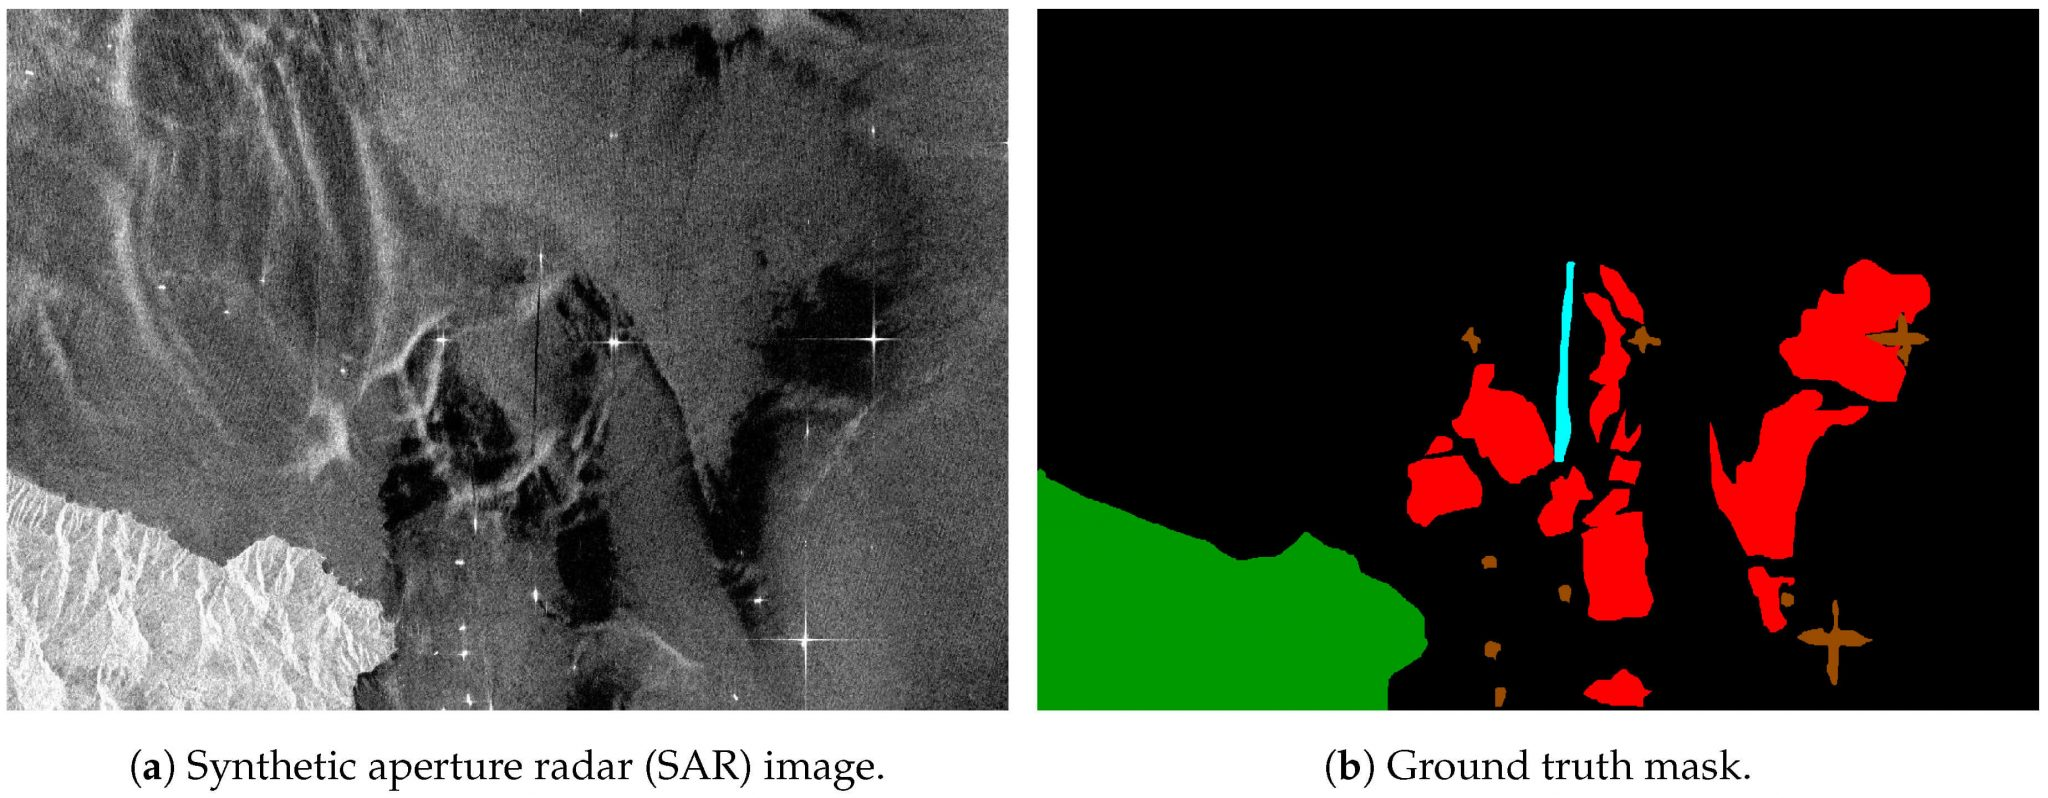
\includegraphics[scale=0.2]{img/section_04/oil_spill_dataset.jpg}
%        \caption{Oil Spill Dataset}
%        \label{fig:section2_oil_spill_dataset}
%    \end{figure}
%\end{frame}
%
%\begin{frame}
%\frametitle{Oil Spill Dataset}
%    Oil Spill Identification from Satellite Images Using Deep Neural Network
%    \cite{rs11151762}
%    \begin{figure}
%        \centering
%        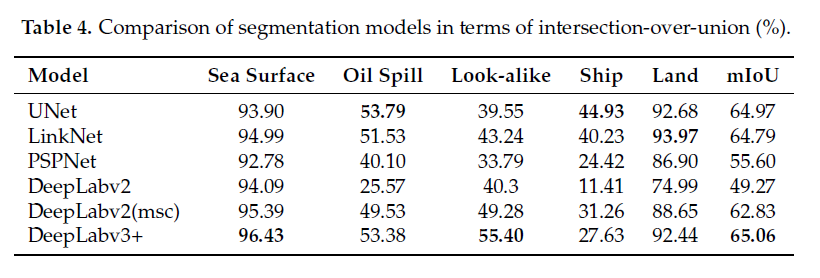
\includegraphics[scale=0.5]{img/section_04/krestenitis_results.png}
%        \caption{Resultados Oil Spill Dataset}
%        \label{fig:section2_oil_spill_dataset}
%    \end{figure}
%\end{frame}
%
%\begin{frame}
%\frametitle{CHN6-CUG}
%    A Global Context-aware and Batch-independent Network for road extraction from VHR satellite imagery
%    \cite{Zhu2021AGC}
%    \begin{figure}
%        \centering
%        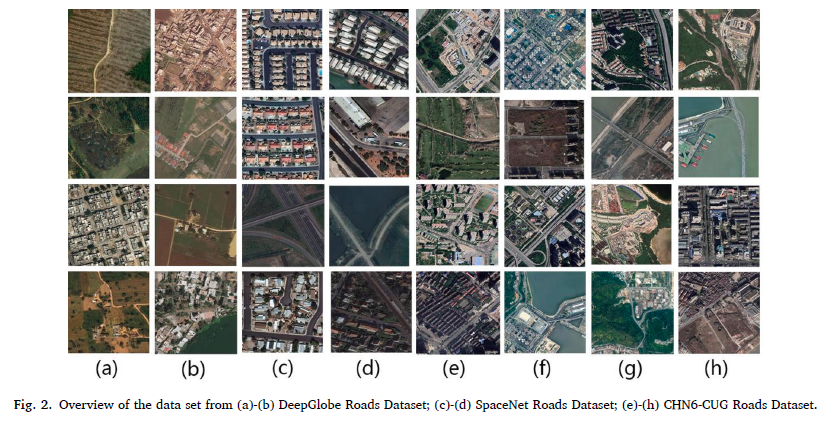
\includegraphics[scale=0.6]{img/section_04/chn6_01.png}
%        \caption{CHN6-CUG}
%        \label{fig:section2_chn6}
%    \end{figure}
%\end{frame}
%
%\begin{frame}
%\frametitle{SOS}
%    Oil Spill Contextual and Boundary-Supervised Detection Network Based on Marine SAR Images
%    \cite{9568691}
%    \begin{figure}
%        \centering
%        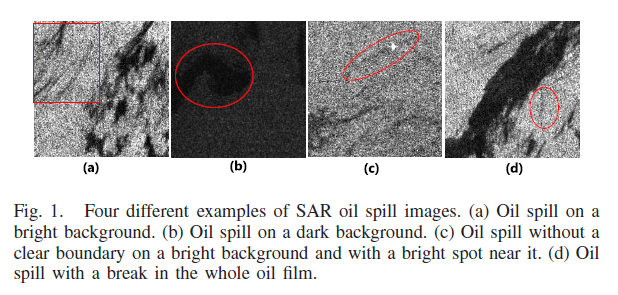
\includegraphics[scale=0.6]{img/section_04/sos_01.png}
%        \caption{SOS}
%        \label{fig:section2_sos}
%    \end{figure}
%\end{frame}
%
%\begin{frame}
%\frametitle{SOS}
%    Oil Spill Contextual and Boundary-Supervised Detection Network Based on Marine SAR Images
%    \cite{9568691}
%    \begin{figure}
%        \centering
%        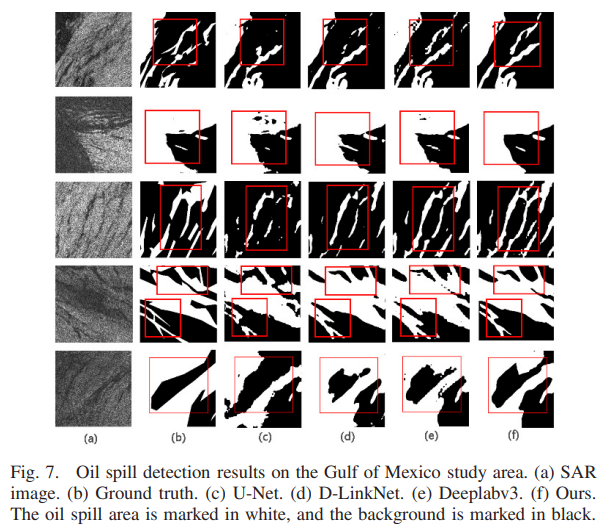
\includegraphics[scale=0.4]{img/section_04/sos_segmentation_01.png}
%        \caption{SOS}
%        \label{fig:section4_sos_segmentation_01}
%    \end{figure}
%\end{frame}
%
%\begin{frame}
%\frametitle{SOS}
%    Oil Spill Contextual and Boundary-Supervised Detection Network Based on Marine SAR Images
%    \cite{9568691}
%    \begin{figure}
%        \centering
%        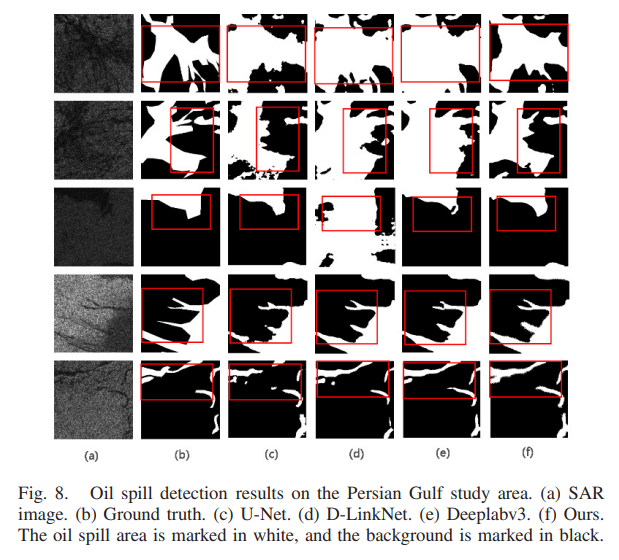
\includegraphics[scale=0.4]{img/section_04/sos_segmentation_02.png}
%        \caption{SOS}
%        \label{fig:section4_sos_segmentation_02}
%    \end{figure}
%\end{frame}
%
%\begin{frame}{Dataset CIMAT}
%    Preprocesamiento de canales de varianza y campo de viento para complementar la información de la imagen original (SAR) con los valores de la retrodispersión
%
%    \begin{figure}
%        \centering
%        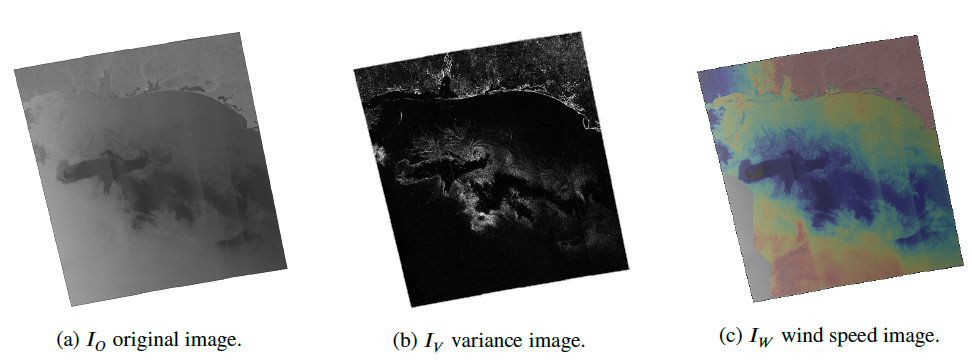
\includegraphics[scale=0.5]{img/section_04/canales.png}
%        \caption{Canales de entrada}
%        \label{fig:my_label}
%    \end{figure}
%\end{frame}
%
%\begin{frame}{Campo de viento}
%    \footnotesize
%    \begin{itemize}
%        \item El campo de viento proporciona información asociada a la rugosidad superficial del océano, ya que si existe poca intensidad de viento las manchas podrán ser visibles teniendo un fondo oscuro mas homogéneo.
%        \item Si la intensidad del viento es demasiado alta la mancha se dispersa y se degrada en el océano.
%    \end{itemize}
%
%    \begin{figure}
%        \centering
%        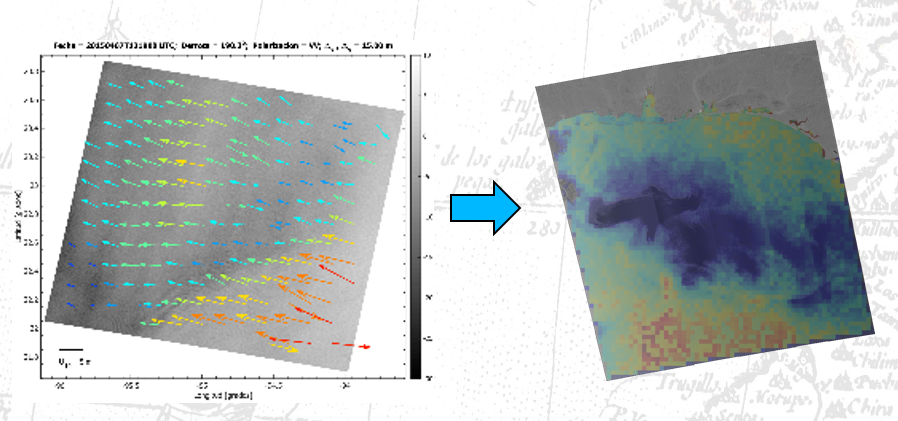
\includegraphics[scale=0.3]{img/section_04/campo_viento.png}
%        \caption{Campo de viento}
%        \label{fig:enter-label}
%    \end{figure}
%\end{frame}
%
%\begin{frame}{Subimágenes}
%    \begin{figure}
%        \centering
%        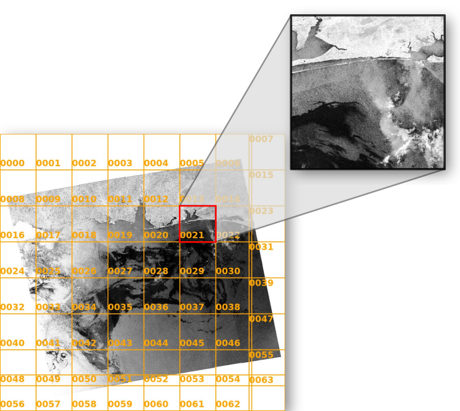
\includegraphics[scale=0.4]{img/section_04/subimagenes.png}
%        \caption{Generación de subimágenes}
%        \label{fig:enter-label}
%    \end{figure}
%\end{frame}
%
%\begin{frame}
%\frametitle{Segmentación Multicanal}
%    \begin{figure}
%        \centering
%        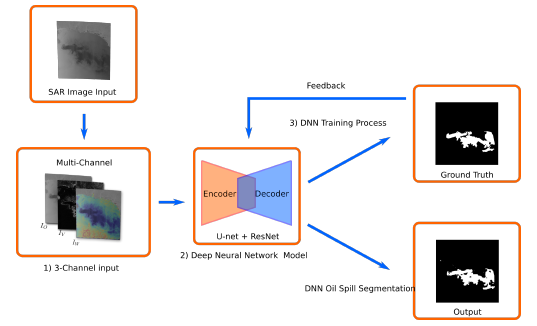
\includegraphics[scale=0.5]{img/section_04/pipeline.png}
%        \caption{Esquema general de la segmentación}
%        \label{fig:my_label}
%    \end{figure}
%\end{frame}
%
